% Alles zur Hardware und unseren Modifikationen
% Zuständig: Mihael
\chapter{Hardware}
\initials{MS}
\label{sec:hardware}
\section{Elegoo Tumbller Kit}
\initials{MS}
\label{subsec:elegoo_tumbller}
Um den Hardwareaufbau so einfach wie möglich zu gestalten,
entschieden wir uns dafür,
fertig entwickelte Kits online zu bestellen und dann zu modifizieren.
%
Die Wahl des Kits fiel letztendlich auf den ``Tumbller'' von Elegoo (Siehe Abbildung \ref{fig:elegoo_tumbller}).
%
Der Tumbller ist ein zweirädriger Roboter, welcher auf einer Achse balanciert.
%
Zur Steuerung des unmodifizierten Kits gibt es eine Smartphone-App,
welche die Roboter über Bluetooth fernsteuern kann.
%
Da wir die Roboter stattdessen über WLAN steuern wollten, 
und die Tumbller-Kits standardmäßig nur ein Bluetooth-Modul eingebaut haben,
haben wir die mitgelieferten Arduino Nano durch ESP32-Boards im Arduino Nano-Format ersetzt.
% TODO Spannungsunterschiede Arduino Nano vs ESP
\begin{figure}[H]
    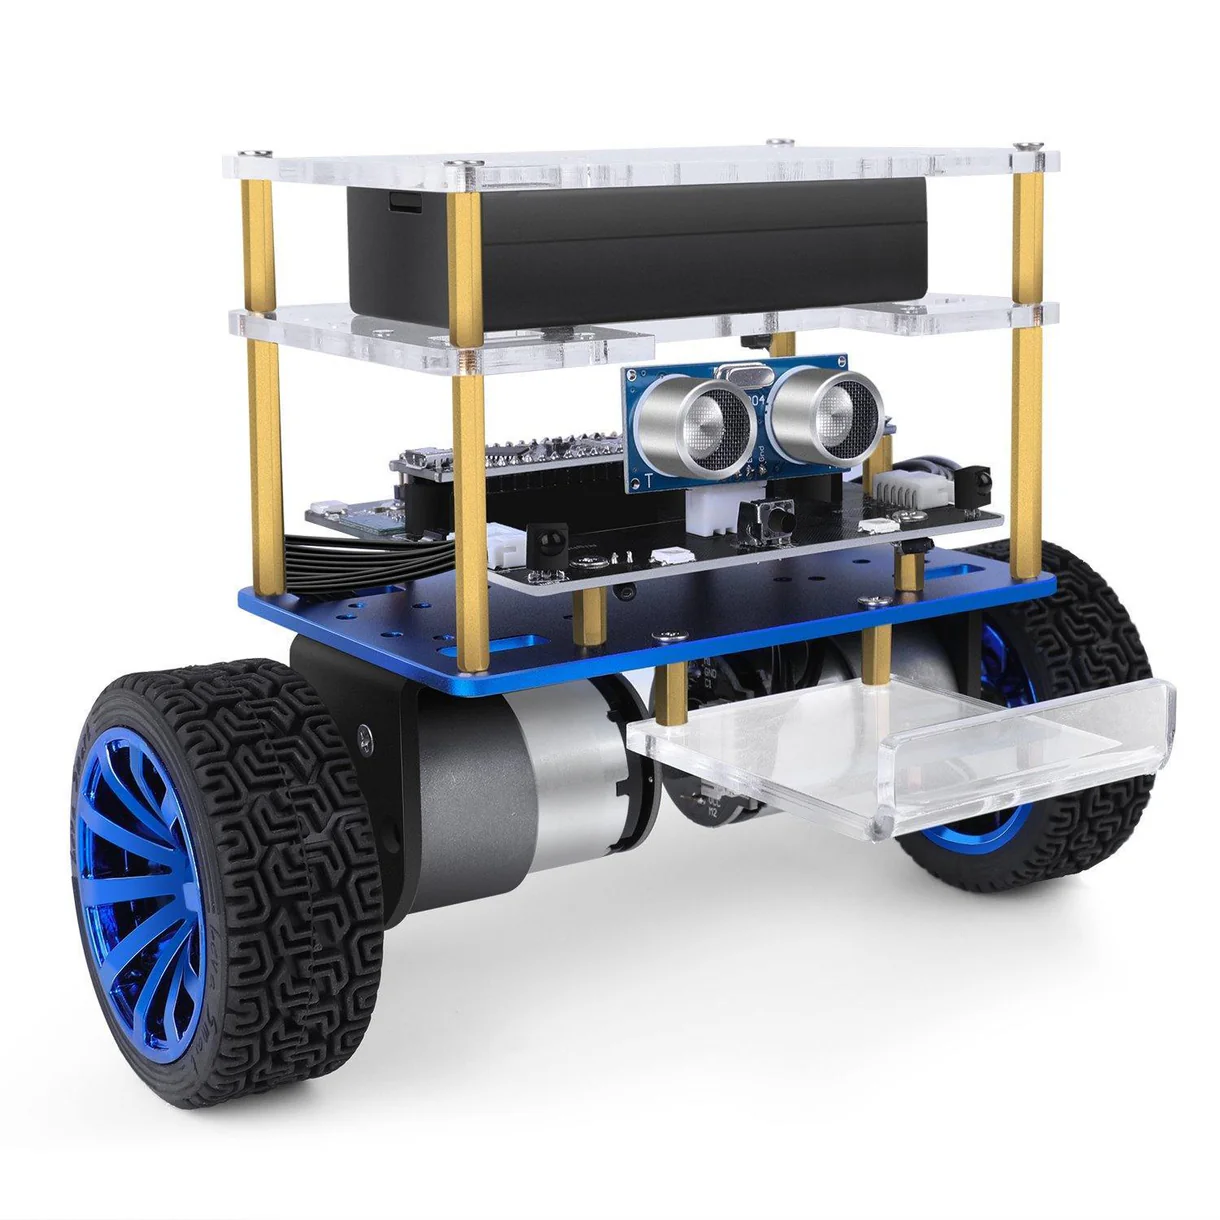
\includegraphics[width=0.7\textwidth, center]{img/elegoo_tumbller.png}
    \caption{Rendering des Elegoo Tumbller}
    \label{fig:elegoo_tumbller}
\end{figure}

% TODO der ganze Absatz muss neu strukturiert werden
Wie in Abbildung \ref{fig:elegoo_tumbller} zu sehen ist,
besteht der unmodifizierte Elegoo Tumbler aus einem Arduino Nano,
der zur Steuerung des gesamten Roboters verwendet wird.
%
Einem MPU6050 (Gyroskop- \& Beschleunigungssensor),
der zur Erkennung der Achsen und Bewegungen verwendet wird (balancieren).
%
Des Weiteren hat er auch zwei Gleichstrommotoren mit Hall-Encodern zur Messung der Raddrehung,
diese Motoren werden mit dem TB6612FNG Motortreiber gesteuert.
%
Zudem verfügt der Elegoo Tumbler über ein HC-06 Bluetooth-Modul,
das zur Kommunikation mit dem Smartphone verwendet wird.
%
Mithilfe des SR04 Ultraschallsensor ist der Roboter in der Lage,
Abstände zu messen, was es ihm ermöglicht, Hindernisse zu erkennen und zu umgehen.
%
Zudem besitzt der Tumbler Infrarot-Sensoren (IR204C-A und IRM-56384), die es ihm ermöglichen,
Hindernisse und Linien zu erkennen oder zu verfolgen.
%
Durch den AMS1117 3.3V Spannungswandler wird die Spannung von dem Li-Ion-Akku,
der als Hauptstromversorgung dient, heruntergestuft,
sodass sie auch für das Bluetooth-Modul und die Sensoren verwendbar ist.
%
Des Weiteren ist der Elegoo Tumbler mit mehreren Modi ausgestattet.
%
Diese kann man entweder über die App oder direkt am Roboter über einen Taster steuern,
zur Visualisierung der Modi hat der Elegoo Tumbler mehrere LEDs eingebaut.
\section{Subkomponenten}
\initials{MS}
\label{subsec:subkomponenten}
%
\subsection{PCB}
\initials{MS}
%
\subsubsection{Allgemein}
\initials{MS}
Das PCB (Printed Circuit Board) im originalen Elegoo Tumbller ist eine fertig entwickelte Leiterplatte,
wie in Abbildung \ref{fig:elegoo_tumbller_original_circuit} zu sehen ist.
%
Auf dieser Leiterplatte sind alle elektronischen Bauteile des Roboters aufgebaut.
%
Die einzelnen Komponenten müssen nur noch in die vorgesehenen Sockel gesteckt werden.
%
\subsubsection{Technische Umsetzung}
\initials{MS}
% TODO redundant v
Die Leiterplatte im originalen Elegoo Tumbller besteht aus mehreren Leiterbahnen.
% TODO unnötig v
Diese Leiterbahnen sind feine Kupferstreifen,
die dafür sorgen,
dass alle elektronischen Bauteile miteinander verbunden sind.
%
Auf der PCB befinden sich alle wichtigen Anschlüsse und Lötpunkte,
die für den Betrieb des Roboters notwendig sind. Dazu gehören:
\begin{itemize}
    \item Steckplätze für den Arduino Nano
    \item Anschlussbuchsen für die beiden Motoren
    \item Steckplätze für die Sensoren (MPU6050, Ultraschallsensor, Infrarot-Sensoren)
    \item Anschluss für das Bluetooth-Modul (HC-06)
    \item Taster für die Modus-Auswahl
    \item LEDs zur Anzeige des Betriebszustands
    \item Lötpads für die Stromversorgung (Li-Ion Akku)
    \item Anschluss für den AMS1117 Spannungsregler
\end{itemize}
% TODO redundant v
Die Leiterbahnen sind so angeordnet,
dass der Strom von der Stromquelle zu allen Bauteilen auf der Platine verteilt wird.
%
Außerdem hat die PCB eigene Lötpunkte für die Motorsteuerung.
%
Der TB6612FNG Motortreiber ist direkt auf der Platine verlötet und sorgt dafür,
dass die beiden Motoren in beide Richtungen gesteuert werden können.
%
\subsubsection{Vorteile}
\initials{MS}
Die originale PCB im Elegoo Tumbller bringt mehrere Vorteile mit sich.
%
Durch die fertig entwickelte Platine können alle Bauteile einfach angeschlossen werden,
ohne dass zusätzliche Drähte verlötet werden müssen.
%
Dadurch bleibt der Aufbau übersichtlich und ordentlich.
%
Die PCB ist kompakt aufgebaut,
wodurch der Platz im Roboter optimal genutzt wird.
%
Zusätzlich sind auf der Platine LEDs vorhanden,
die den aktuellen Betriebszustand anzeigen können.
%
Da alle Verbindungen direkt auf der Leiterplatte verlaufen,
gibt es weniger Möglichkeiten für Wackelkontakte oder lockere Verbindungen.

\subsubsection{Einschränkungen}
\initials{MS}
Die PCB des originalen Tumbller ist nur für die mitgelieferten Komponenten ausgelegt.
%
Wenn man zusätzliche Sensoren oder einen anderen Mikrocontroller (wie im SwarmBots-Projekt) verwenden möchte,
muss die die Platine modifiziert werden,
was schnell zu einer komplexen Aufgabe werden kann.
%
Siehe Abbildung \ref{fig:elegoo_tumbller_original_circuit} auf Seite \pageref{fig:elegoo_tumbller_original_circuit}.
%
\begin{sidewaysfigure}
    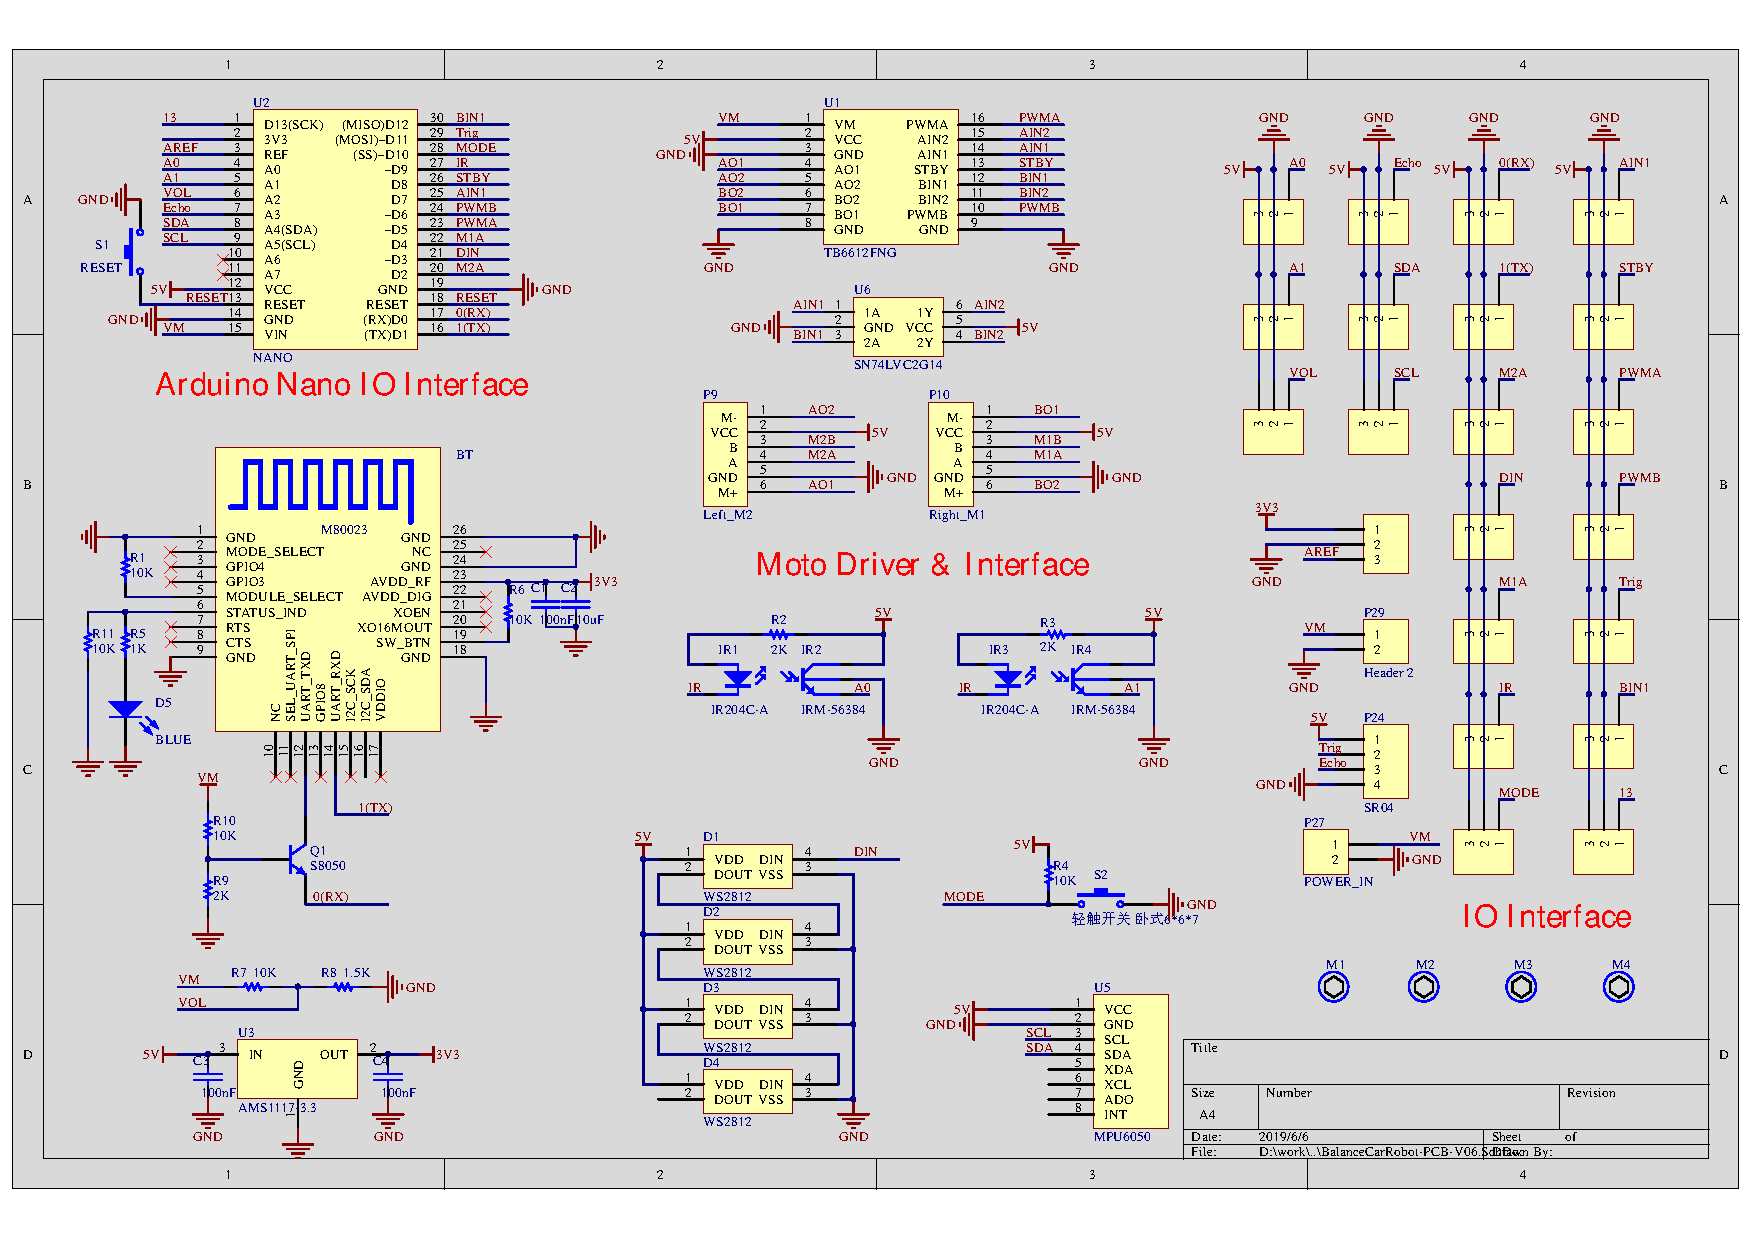
\includegraphics[width=\textwidth, center]{img/elegoo_tumbller_original_circuit.pdf}
    \caption{Originaler Schaltplan des Tumbllers (TODO: neu zeichnen)}
    \label{fig:elegoo_tumbller_original_circuit}
\end{sidewaysfigure}
%
\newpage
\subsection{MPU6050 (Gyroskop- \& Beschleunigungssensor)}
\initials{MS}
%
\subsubsection{Allgemein}
\initials{MS}
Der MPU6050 ist ein 6-Achsen-Sensor,
der aus einem Drehratensensor (Gyroskop, welcher Drehbewegungen in 3 Achsen misst)
und einem Beschleunigungssensor (Accelerometer, welcher lineare Beschleunigungen in 3 Achsen misst),
wie in Abbildung \ref{fig:mpu6050} zu sehen ist.
\subsubsection{Technische Daten}
\initials{MS}
\begin{figure}[H]
    \centering
    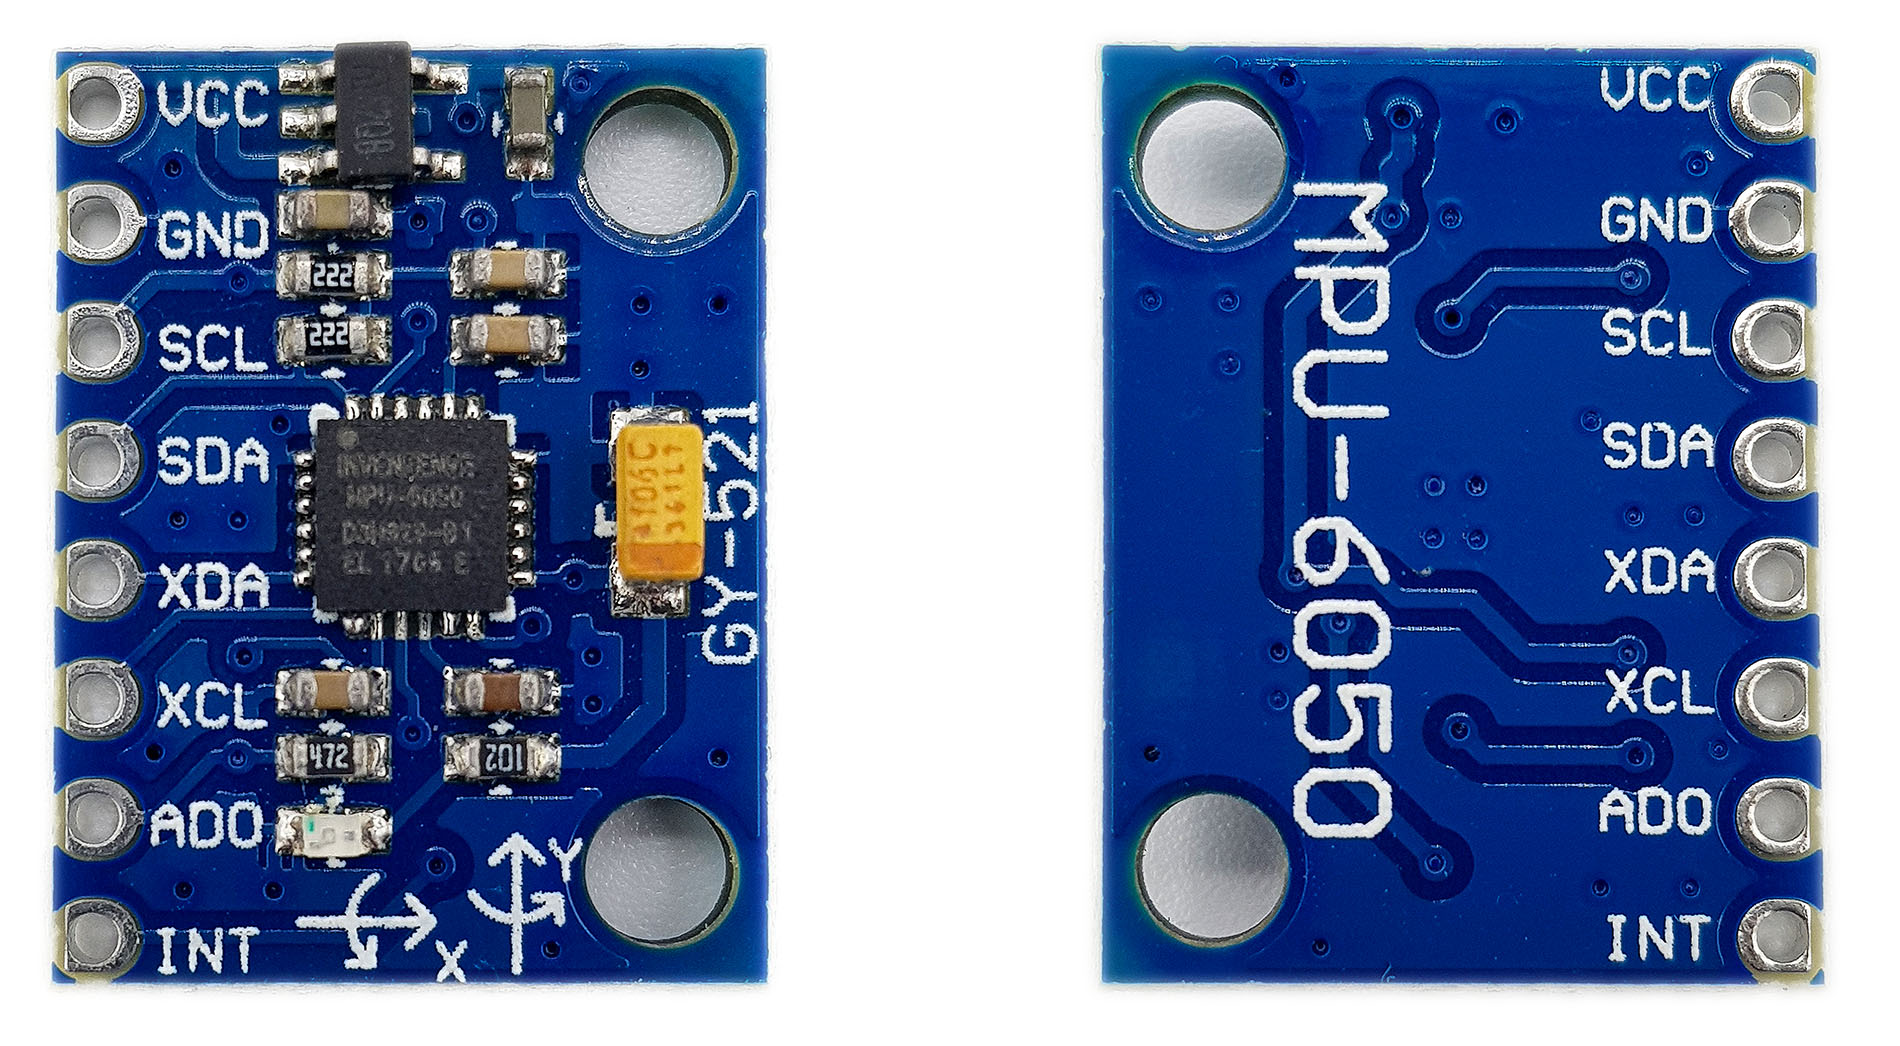
\includegraphics[width=0.7\textwidth]{img/Hardware/MPU6050.png}
    \caption{MPU6050 Gyroskop- und Beschleunigungssensor}
    \label{fig:mpu6050}
\end{figure}
Als Betriebsspannung verwendet der MPU6050 2,3V bis 3,4V,
als Kommunikationsprotokoll verwendet er I2C oder SPI (I2C Standard: 0x68 Adresse).
%
Der Messbereich des Gyroskops und Accelerometers kann konfiguriert werden
(Gyroskop:  ±250, ±500, ±1000, ±2000 °/s, Accelerometer: ±2g, ±4g, ±8g, ±16g),
durch die Konfigurationsmöglichkeit ergeben sich auch unterschiedliche Empfindlichkeiten der beiden
(Gyroskop: 131 LSB/°/s (bei ±250 °/s),
Accelerometer: 16.384 LSB( least significant bit/ niedrigstes Bit)/g (bei ±2g)).
%
Die Genauigkeit der beiden liegt bei ca. ±0,01 °/s für den Gyroskop-Sensor und ca. ±0,005g für den Accelerometer.
%
Der MPU6050 über eine Abtastrate von bis zu 1kHz und über einen integrierten DMP (Digital Motion Processor),
welcher es ermöglicht, Datenfusion durchzuführen.
%
\subsubsection{Einschränkungen}
\initials{MS}
Der Gyroskop-Sensor hat einen Drift,
der dazu führt, dass sich die Messwerte bei längerer Laufzeit verschieben.
%
Zudem reagiert der MPU6050 empfindlich auf Vibrationen,
wodurch Messfehler entstehen können.
%
\subsection{TB6612FNG (Motortreiber)}
\initials{MS}
%
\subsubsection{Allgemein}
\initials{MS}
Der TB6612FNG ist ein Dual-H-Brücke-Motortreiber,
welcher verwendet wird,
um einen Schrittmotor oder zwei Gleichstrommotoren wie beim Tumbler zu steuern.
%
Der Motortreiber ermöglicht es,
Gleichstrommotoren in zwei Richtungen zu betreiben,
wie in Abbildung \ref{fig:motortreiber} dargestellt.
%
\subsubsection{Technische Daten}
\initials{MS}
\begin{figure}[H]
    \centering
    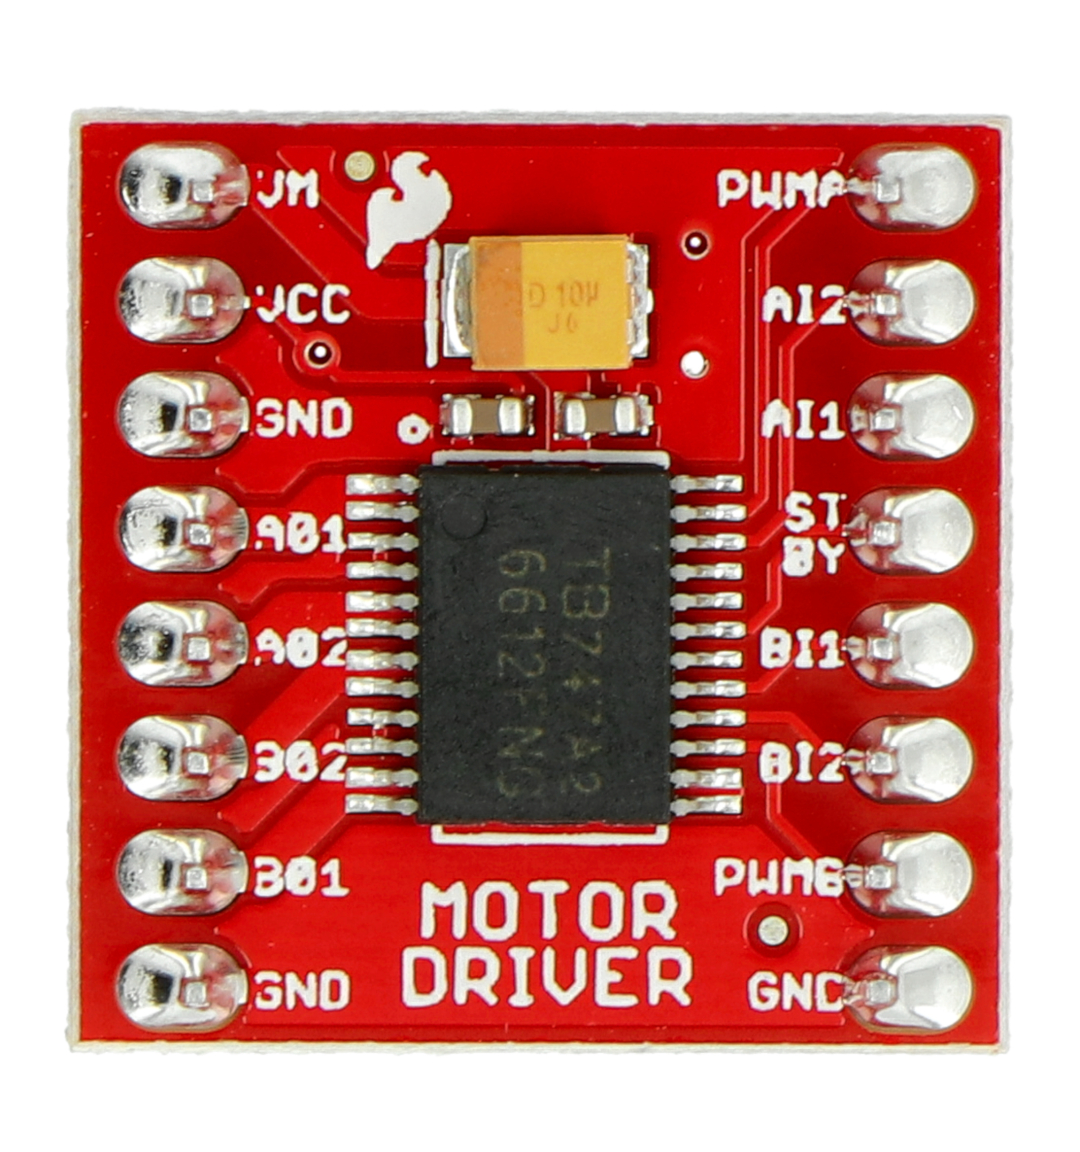
\includegraphics[width=0.3\textwidth]{img/Hardware/Motortreiber.png}
    \caption{TB6612FNG Motortreiber}
    \label{fig:motortreiber}
\end{figure}
Als Versorgungsspannung für Motoren kann der TB6612FNG 2,5V bis 13,5V ausgeben,
für die Logik ist die Versorgungsspannung 2,7V bis 5,5V.
%
Der maximale Ausgangsstrom ist 1,2 A (kontinuierlich), 3 A (kurzzeitig pro Kanal),
er besitzt 2 Kanäle und als Steuersignal verwendet er PWM (Pulsweitenmodulation) und Richtungssignale.
%
Zudem besitzt er eine integrierte Schutzschaltung,
die vor Überstromschutz, Übertemperaturschutz und Kurzschlussschutz schützt. 
%
Die Verlustleistung ist sehr gering,
da der Motortreiber die MOSFET-Technologie verwendet.
%
(MOSFET (Metal Oxide Semiconductor Field Effect Transistor) ist ein elektronisches Bauteil, 
das wie ein elektronischer Schalter funktioniert und in der Motorsteuerung verwendet wird,
um mit einem kleinen Steuersignal einen großen Stromfluss für Motoren zu kontrollieren)
\subsubsection{Belegung}
\initials{MS}
Pin	-	Funktion
VM	Versorgungsspannung für die Motoren (2,5–13,5V)
VCC	Logik-Spannungsversorgung (2,7–5,5V)
GND	Masse (gemeinsames Minus)
AIN1	Richtungssignal Motor A (Logik-Eingang)
AIN2	Richtungssignal Motor A (Logik-Eingang)
PWMA	PWM-Signal für Geschwindigkeit Motor A
BIN1	Richtungssignal Motor B (Logik-Eingang)
BIN2	Richtungssignal Motor B (Logik-Eingang)
PWMB	PWM-Signal für Geschwindigkeit Motor B
STBY	Standby-Pin (aktiv bei HIGH)
AO1	Ausgang Motor A (Pluspol)
AO2	Ausgang Motor A (Minuspol)
BO1	Ausgang Motor B (Pluspol)
BO2	Ausgang Motor B (Minuspol)

\subsubsection{Ansteuerung}
\initials{MS}
Durch die Kombination Richtungssignale (AIN1, AIN2 / BIN1, BIN2),
kann der Motor entweder vorwärts-, rückwärtsfahren oder anhalten.
%
Der PWMA-/PWMB-Eingang wird verwendet, um die Geschwindigkeit zu steuern.
%
\subsection{AMS1117 (3.3V Spannungsregler)}
\initials{MS}
%
\subsubsection{Allgemein}
\initials{MS}
Der AMS1117 ist ein linearer Spannungsregler,
der aus einer höheren Eingangsspannung eine stabile kleinere Ausgansspannung (3,3V) macht.
%
Im Elegoo Tumbller wird er verwendet,
um die Spannung auf 3,3 Volt zu reduzieren.
%
Diese Spannung brauchen einige Bauteile,
wie zum Beispiel das Bluetooth-Modul,
damit sie nicht kaputtgehen.
%
Wie in Abbildung \ref{fig:ams1117} dargestellt,
ist der Spannungsregler direkt auf der Platine integriert.
\subsubsection{Technische Daten}
\initials{MS}
\begin{figure}[H]
    \centering
    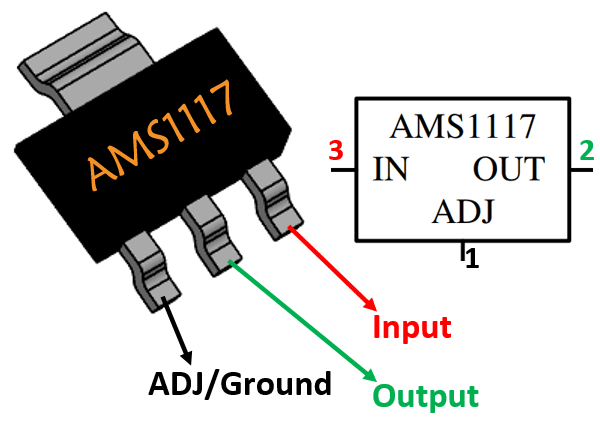
\includegraphics[width=0.6\textwidth]{img/Hardware/AMS1117.png}
    \caption{AMS1117 Spannungsregler}
    \label{fig:ams1117}
\end{figure}
Der Spannungsregler kann mit 4,5V bis 15V betrieben werden,
er hat eine fixe Ausgansspannung von 3,3V und kann maximal 1A Ausgangstrom liefern (mit einer Kühlung),
die Drop-out Spannung beträgt 1,1V (bei 1A).
%
Es gibt einen integrierten Übertemperatur- und Kurzschlussschutz.
%
\subsection{HC-06 (Bluetooth Modul)}
\initials{MS}
%
\subsubsection{Allgemein}
\initials{MS}
Das HC-06 ist ein Bluetooth-Modul,
das es ermöglicht,
mittels Bluetooth Daten zu übertragen.
%
Wie in Abbildung \ref{fig:hc06} zu sehen ist,
ist das Modul sehr kompakt aufgebaut.
\subsubsection{Technische Daten}
\initials{MS}
\begin{figure}[H]
    \centering
    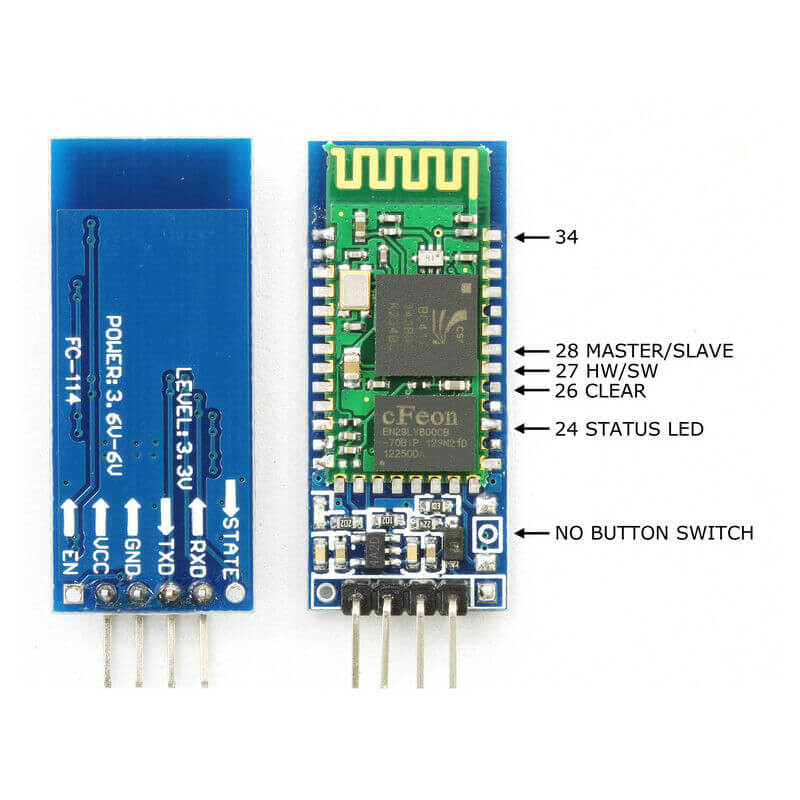
\includegraphics[width=0.6\textwidth]{img/Hardware/hc06.png}
    \caption{HC-06 Bluetooth-Modul}
    \label{fig:hc06}
\end{figure}
Das Bluetooth Modul wird mit einer Betriebsspannung von 3,3V betrieben.
Als Kommunikationsmethode verwendet es UART 
(UART (Universal Asynchronous Receiver Transmitter) ist eine serielle Schnittstelle,
die Daten bitweise und ohne Taktsignal zwischen zwei Geräten über nur zwei Leitungen (TX und RX) überträgt.).
%
Die Version, die es unterschütz ist, Bluetooth 2.0 + EDR, es hat eine Reichweite von bis zu ca. 10m und hat eine Datenrate von bis zu 2,1 Mbps.
%
Als Funkfrequenz verwendet es sdas 2,4 GHz Band, die Sicherheitsfunktion,
die man einschalten kann, erfordert es einen Pin-Code vor der Verbindung einzugeben.
%
Das HC-06 ferfügt nur über den Slave-Modus.
%
(Der Slave-Modus bedeutet, dass ein Gerät keine Verbindung selbst starten kann,
sondern nur auf Verbindungsanfragen von anderen Geräten wartet und dann darauf reagiert.)
\subsubsection{Belegung}
\initials{MS}
Pin	-	Funktion
VCC	Versorgungsspannung (3,3V)
GND	Masse
TXD	Sendedaten (wird mit RX des Arduino verbunden)
RXD	Empfangsdaten (wird mit TX des Arduino verbunden)
STATE	Verbindungsstatus-Ausgang (optional)

\subsubsection{Einschränkungen}
\initials{MS}
Durch die veraltete Bluetooth-Version ist nur eine niedrigere Datenrate möglich
und es besteht eine höhere Störanfälligkeit als bei modernen Standards.
%
\subsection{Arduino Nano (Microcontroller)}
\initials{MS}
%
\subsubsection{Allgemein}
\initials{MS}
Der Arduino Nano ist einer der kleineren (ca. 18 x 45 mm) uC (Mikrocontroller),
dieser wurde verwendet, um alle elektronischen Bauteile im Tumbler zu steuern.
%
Wie in Abbildung \ref{fig:arduino_nano} zu sehen ist,
wird der Arduino Nano direkt auf der PCB eingesteckt und bildet die zentrale Steuerungseinheit des Roboters.
\subsubsection{Technische Daten}
\initials{MS}
\begin{figure}[H]
    \centering
    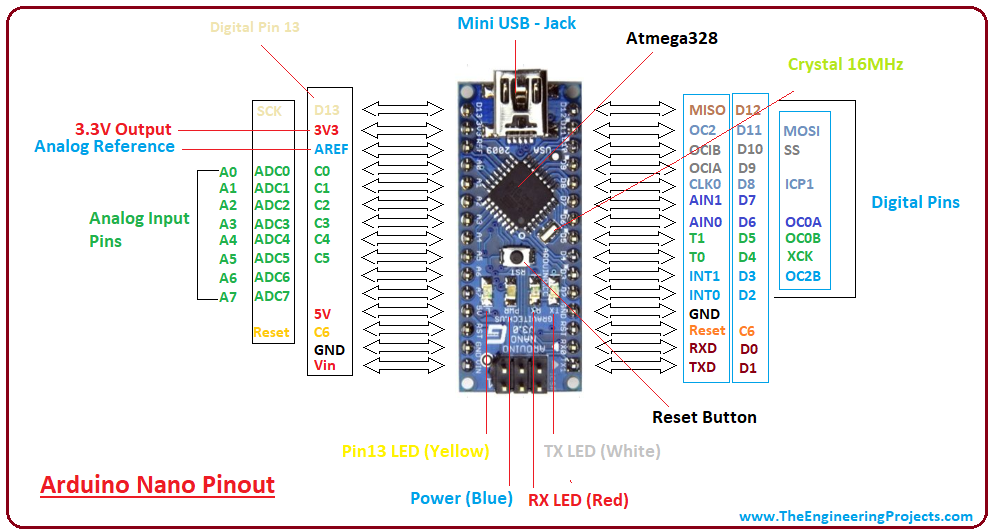
\includegraphics[width=1\textwidth]{img/Hardware/arduino_nano.png}
    \caption{Arduino Nano Mikrocontroller}
    \label{fig:arduino_nano}
\end{figure}
Der Arduino Nano hat einen ATmega328P als Prozessor und eine Taktfrequenz von 16MHz.
%
Die Betriebsspannung beträgt 5V (Versorgungspannung über den Pin VIN 7V bis 12V). 
Er besitzt 14 Digitale i/O Pins (Input/Output),
wobei 6 davon PWM fähig sind.
%
Zudem besitz er 8 Analoge Pins und einen Flash-Speicher von 32KB (davon 2 KB für Bootloader). 
%
Der SRAM hat 2KB und das EEPROM 1KB. Die Schnittstellen, die er unterschützt, sind UART, I2C, SPI.
%
UART (Universal Asynchronous Receiver Transmitter)
UART ist eine serielle Schnittstelle, die Daten bitweise über zwei Leitungen (TX für Senden und RX für Empfangen) überträgt.
%
Dabei wird kein Taktsignal verwendet -- beide Geräte müssen die gleiche Geschwindigkeit (Baudrate) eingestellt haben.
%
I2C (Inter-Integrated Circuit)
I2C ist ein Kommunikationsprotokoll,
das mehrere Geräte über nur zwei Leitungen verbindet:
eine Datenleitung (SDA) und eine Taktleitung (SCL).
%
Ein Gerät ist der Master (Steuergerät), die anderen sind Slaves (empfangen Befehle).
%
SPI (Serial Peripheral Interface)
SPI ist eine serielle Schnittstelle für den schnellen Datenaustausch zwischen einem Master und einem oder mehreren Slave-Geräten.
%
Es werden vier Leitungen verwendet:
MOSI (Daten vom Master zum Slave),
MISO (Daten vom Slave zum Master),
SCK (Taktsignal)
und SS (Slave Select, Auswahl des Geräts).
\subsubsection{Belegung}
\initials{MS}
(TODO Bild)
\subsubsection{Einschränkungen}
\initials{MS}
Der Arduino-Nano besitzt ein kleiner Speicher was ihn nicht geeignet macht für komplexen Programmen, die viel Speicher benötigen.
%
Zudem hat er nur einen 8-Bit-Prozessor, was ihn auch in der Rechenleistung stark begrenzt.
%
Außerdem hat er kein integriertes WLAN-Modul, 
was es nur ermöglicht ihn  über Kabel oder Bluetooth zu verwenden.
%
\subsection{SR04 (Ultraschallsensor)}
\initials{MS}
%
\subsubsection{Allgemein}
\initials{MS}
Der SR04 ist ein Ultraschallsensor,
der verwendet wird, um den Abstand zu Objekten zu messen.
%
Er sendet einen Ultraschallton aus,
dieser wird von einem Hindernis reflektiert,
und der Sensor misst die Zeit,
bis das Echo zurückkommt,
wie in Abbildung \ref{fig:sr04} dargestellt.
\subsubsection{Technische Daten}
\initials{MS}
\begin{figure}[H]
    \centering
    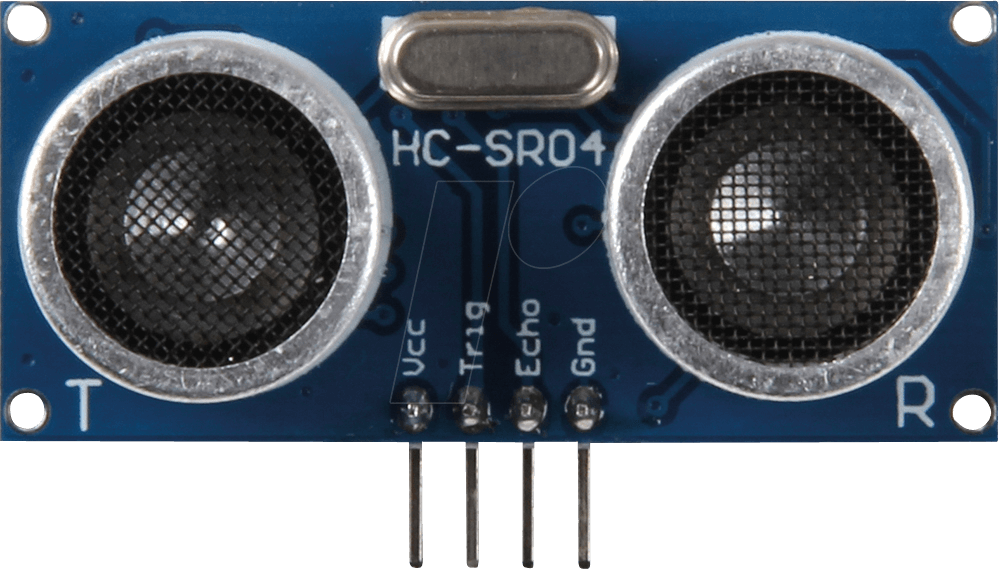
\includegraphics[width=0.7\textwidth]{img/Hardware/sr04.png}
    \caption{SR04 Ultraschallsensor}
    \label{fig:sr04}
\end{figure}
Der SR04 hat eine Betriebsspannung von 5V und eine Stromaufnahme von ca. 15mA.
%
Zudem hat er einen Messbereich von 2cm bis 400cm und eine Genauigkeit von ca. ±3 mm.
%
Sein Messwinkel beträgt 15°
und er hat als Ausgänge den Trigger-Pin (Signal senden) und Echo-Pin (Signal empfangen). 
%
Die Frequenz mit der er arbeitet, sind 40 kHz (Ultraschall).
\subsubsection{Belegung}
\initials{MS}
Pin  -   	Funktion
VCC	Versorgungsspannung (5V)
GND	Masse
Trig	Trigger-Eingang → Startet das Signal
Echo	Echo-Ausgang → Gibt das empfangene Signal weiter
\subsubsection{Einschränkungen}
\initials{MS}
Der Ultraschallsensor ist sehr empfindlich
gegenüber schrägen Flächen und arbeitet relativ langsam,
was ihn ungeeignet für bestimmte Orte und Aufgaben macht.
%
Zudem kann er bei Objekten unter 2cm Entführung keine Messung machen.
%
\subsection{Infrarot-Sensoren (IR204C-A \& IRM-56384)}
\initials{MS}
%
\subsubsection{Allgemein}
\initials{MS}
Die Infrarot-Sensoren IR204C-A und IRM-56384 werden im Elegoo Tumbller verwendet,
um Hindernisse und Linien zu erkennen.
%
Sie funktionieren mit unsichtbarem Infrarotlicht (kurz: IR)
und arbeiten nach dem Reflexionsprinzip,
wie in Abbildung \ref{fig:infrarot_sensoren} zu sehen ist.
\subsubsection{Technische Daten}
\initials{MS}
\begin{figure}[H]
    \centering
    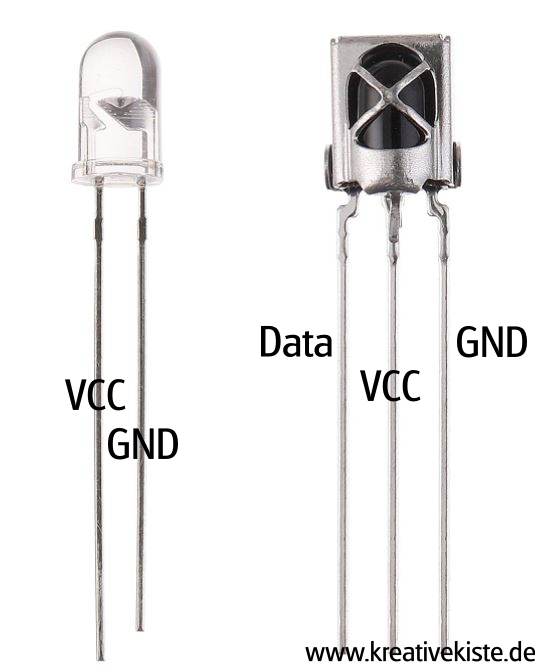
\includegraphics[width=0.4\textwidth]{img/Hardware/Infrarot_Sensor.png}
    \caption{Infrarot-Sensoren IR204C-A und IRM-56384}
    \label{fig:infrarot_sensoren}
\end{figure}
Die Infrarot Sensoren arbeiten mit einer Betriebspannung von 5V und bestehen aus einer Infrarot-LED
(LED, welche Infrarot Licht ausstrahlt) und 
einem Fototransistor (Transistor, welcher auf Licht reagiert).
%
Der Erfassungsbereich liegt bei ca. 1 cm bis 10 cm (je nach Oberfläche),
als Ausgang hat es Digital (HIGH = frei, LOW = Hindernis erkannt).
%
Die Wellenlänge, mit welcher es arbeitet ist ca. 940 nm (unsichtbares Infrarotlicht).

IR204C-A:
Der IR204C-A ist eine Infrarot-LED.
%
Sie sendet unsichtbares Infrarotlicht aus.
%
Dieses Licht wird von Objekten reflektiert,
damit der Roboter erkennen kann, ob ein Hindernis vor ihm steht.

IRM-56384:
Der IRM-56384 ist ein Infrarot-Empfänger.
%
Er empfängt Infrarot-Signale und erkennt,
ob Licht von der Infrarot-LED zurückkommt oder ob ein Signal von einer Fernbedienung gesendet wird.
\subsubsection{Einschränkungen}
\initials{MS}
Da die Infrarot LED nicht stark ist und der Empfänger nicht genau kann es zu Problemen führen bei Tageslicht oder Lampen.
%
Zudem funktionier diese Verfahren nur auf sehr kurzer Distanz (meist unter 10cm),
und das Material welcher als Reflektor dient, kann ein Problem aufweisen da,
Schwarze oder matte Flächen schlechter reflektieren.
%
\subsection{Gleichstrommotoren (TT130 DC Motor mit 1:48 Getriebe)}
\initials{MS}
%
\subsubsection{Allgemein}
\initials{MS}
Im Elegoo Tumbller werden zwei kleine Gleichstrommotoren (DC-Motoren) verwendet.
%
Diese Motoren sind dafür verantwortlich,
die beiden Räder des Roboters anzutreiben.
%
Ein Gleichstrommotor wandelt elektrische Energie in mechanische Bewegung um -- also in eine Drehbewegung.
%
In Abbildung \ref{fig:gleichstrommotor} ist der verwendete Motor zu sehen.

\subsubsection{Technische Daten}
\initials{MS}
\begin{figure}[H]
    \centering
    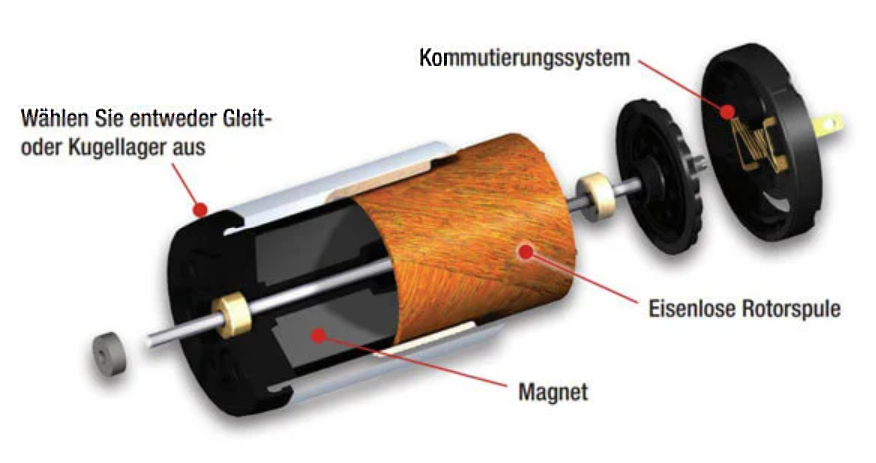
\includegraphics[width=1\textwidth]{img/Hardware/gleichstrommotor.png}
    \caption{TT130 DC Motor mit Getriebe}
    \label{fig:gleichstrommotor}
\end{figure}
Die Gleichstrommotoren haben eine Betriebsspannung von 6V bis 12V und einen Nennstrom von ca. 200mA und sind Bürsten-Gleichstrommotor.
%
(Ein Bürsten-Gleichstrommotor ist ein Motor, der mithilfe von kleinen Bürsten Strom bekommt und sich dadurch dreht)
Die Drehzahl beträgt ca. 300 Umdrehungen pro Minute (RPM).
%
Zudem verfügen sie über ein eingebautes Getriebe zur Erhöhung des Drehmoments und einen Wellen-Durchmesser von 3mm.
%
(Das Drehmoment gibt an,
wie stark er etwas drehen kann,
der Wellen-Durchmesser beschreibt,
wie dick die Achse des Motors ist)
\subsubsection{Funktionsweise}
\initials{MS}
Bei einem Gleichstrommotor wird durch Anlegen einer elektrischen Spannung ein Magnetfeld erzeugt,
welches den Rotor bewegt.
%
Durch Umpolen (Richtungsänderung des Stroms) kann die Drehrichtung geändert werden.
%
Die Geschwindigkeit wird durch PWM-Signale (Pulsweitenmodulation) geregelt,
die Richtung durch digitale Signale. %TODO welche?
%
\subsection{Encoder}
\initials{MS}
\subsubsection{Allgemein}
\initials{MS}
Die Encoder im Elegoo Tumbller sind in den Motoren eingebaut und dienen dazu,
die Drehbewegung der Räder zu messen.
%
Ein Encoder ist ein kleiner Sensor, der erkennt, wie weit und wie schnell sich ein Rad dreht.
%
Damit kann der Roboter berechnen,
wie viel Strecke er zurückgelegt hat oder wie stark sich das Rad gedreht hat --
das ist wichtig für die Stabilität, Steuerung und Navigation.
%
In Abbildung \ref{fig:encoder} ist der Encoder dargestellt.

\subsubsection{Technische Daten}
\initials{MS}
\begin{figure}[H]
    \centering
    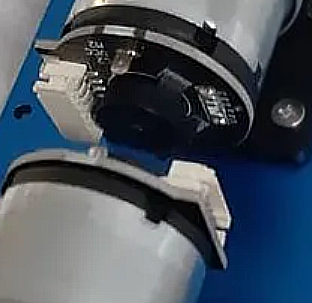
\includegraphics[width=0.5\textwidth]{img/Hardware/encoder.png}
    \caption{Encoder zur Drehzahlmessung}
    \label{fig:encoder}
\end{figure}
Die Encoder sind magnetische Inkremental-Encoder.
Sie arbeiten mit digitalen Impulssiganlen und haben eine Impulszahl von 330 Impulsen pro Rad-Umdrehung.
%
Sie werden mit 5V betrieben und sind direkt am Motor befestigt.
\subsubsection{Funktionsweise}
\initials{MS}
Am Motor ist ein kleiner Magnet eingebaut,
der sich mit dreht.
%
Ein Hall-Effekt-Sensor erkennt jedes Mal,
wenn der Magnet eine bestimmte Stelle passiert,
und sendet einen elektrischer Impuls aus,
welcher dann vom Mikrocontroller ausgewertet wird.
%
Die eingebauten Encoder können nur relative Bewegungen messen,
sie geben keine absolute Position der Räder aus.
%
\subsection{Li-Ion Akku (7,4V)}
\initials{MS}
%
\subsubsection{Allgemein}
\initials{MS}
Der Li-Ion Akku (Lithium-Ionen-Akku) ist die Hauptstromquelle des Roboters.
% 
Er liefert die elektrische Energie, die der Roboter benötigt,
um alle Komponenten wie Motoren, Sensoren und den Mikrocontroller zu betreiben.
%
\subsubsection{Technische Daten}
\initials{MS}
Beim Akku handelt es sich um einen Lithium-Ionen-Akku mit einer Nennspannung von 7,4V.
%
Der Akku besteht aus 2 LiIon-Zellen in Serie (2S), mit jeweils 3,7V Nennspannung pro Zelle.
Die Kapazität des Akkus beträgt ca. 1200 mAh.
%
Zudem ist er gegen Überladung, Tiefentladung und Kurzschlüsse geschützt.
%

\section{Modifikationen}
\initials{MS}
\label{subsec:hardware_modifikationen}

Für das SwarmBots-Projekt mussten die originalen Elegoo Tumbller Roboter technisch verändert werden, damit sie als Schwarm zusammenarbeiten können und über WLAN steuerbar sind.

\subsubsection{Austausch des Mikrocontrollers}
\initials{MS}
Im originalen Tumbller wurde ein Arduino Nano verwendet, der jedoch nur Bluetooth-Kommunikation unterstützt.
%
Für unser Projekt war das nicht ausreichend, weil wir die Roboter über WLAN steuern wollten.
%
Deshalb haben wir die Arduino Nano durch ESP32-Boards im Nano-Format ersetzt.
%
Das ESP32-Board besitzt ein integriertes WLAN-Modul und mehr Rechenleistung.
%
In Abbildung \ref{fig:nanoesp32} ist das verbaute ESP32-Board zu sehen.
%
\begin{figure}[H]
    \centering
    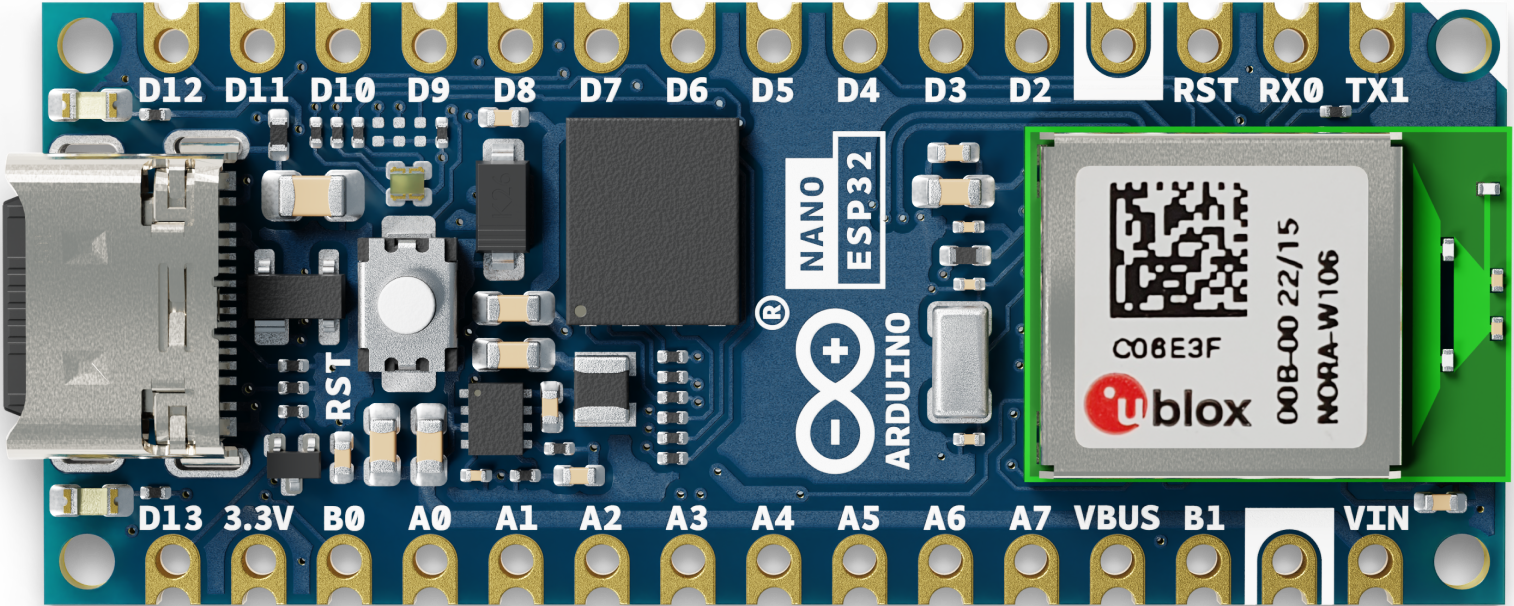
\includegraphics[width=0.6\textwidth]{img/Hardware/nanoesp32.png}
    \caption{ESP32-Board im Nano-Format}
    \label{fig:nanoesp32}
\end{figure}

\subsubsection{Entfernung des Bluetooth-Moduls}
\initials{MS}
Da wir die Kommunikation über WLAN umgestellt haben, wurde das HC-06 Bluetooth-Modul aus allen Robotern entfernt.
%
Die Steuerung per Smartphone-App war dadurch nicht mehr notwendig.

\subsubsection{Anpassung der Stromversorgung}
\initials{MS}
Für die neuen Module (vor allem den LiDAR-Sensor beim Guide-Roboter) musste die Stromversorgung angepasst werden.
%
Dafür haben wir einen zusätzlichen Step-Down-Konverter eingebaut, um eine sichere 5V-Spannung für den Sensor bereitzustellen.
%
Der verbaute Step-Down-Konverter ist in Abbildung \ref{fig:stepdown} dargestellt.

\begin{figure}[H]
    \centering
    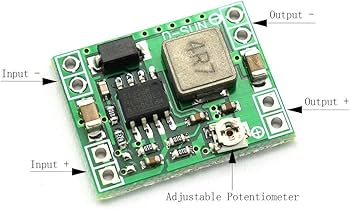
\includegraphics[width=0.6\textwidth]{img/Hardware/stepdown.png}
    \caption{Step-Down-Konverter zur Spannungsanpassung}
    \label{fig:stepdown}
\end{figure}

\subsubsection{Mechanische Änderungen am Guide}
\initials{MS}
Der Guide-Roboter bekam zusätzlich einen LiDAR-Sensor auf der obersten Ebene montiert.
%
Dafür wurde das Chassis verändert:
\begin{itemize}
    \item Die obere Ebene wurde erhöht
    \item Neue Halterungen für den Sensor wurden eingebaut
    \item Das Kabelmanagement wurde angepasst
\end{itemize}
Wie in Abbildung \ref{fig:guide} zu sehen ist,
wurde der LiDAR-Sensor auf der oberen Ebene des Guide-Roboters befestigt.


% Kamera-Integration (ESP32-CAM)
%Alle Roboter wurden mit einem ESP32-CAM-Modul ausgestattet.
% Dadurch können die Roboter Live-Bilder an den Server senden und ihre Umgebung visuell erfassen.



\section{Guide}
\initials{MS}
\label{subsec:hardware_guide}
\subsection{Allgemein}
\initials{MS}
Die Aufgabe von \textit{Guide} ist es,
mithilfe eines LiDAR-Sensors die Umgebung nach Hindernissen und den anderen Robotern abzusuchen.

\begin{figure}[H]
   \centering
   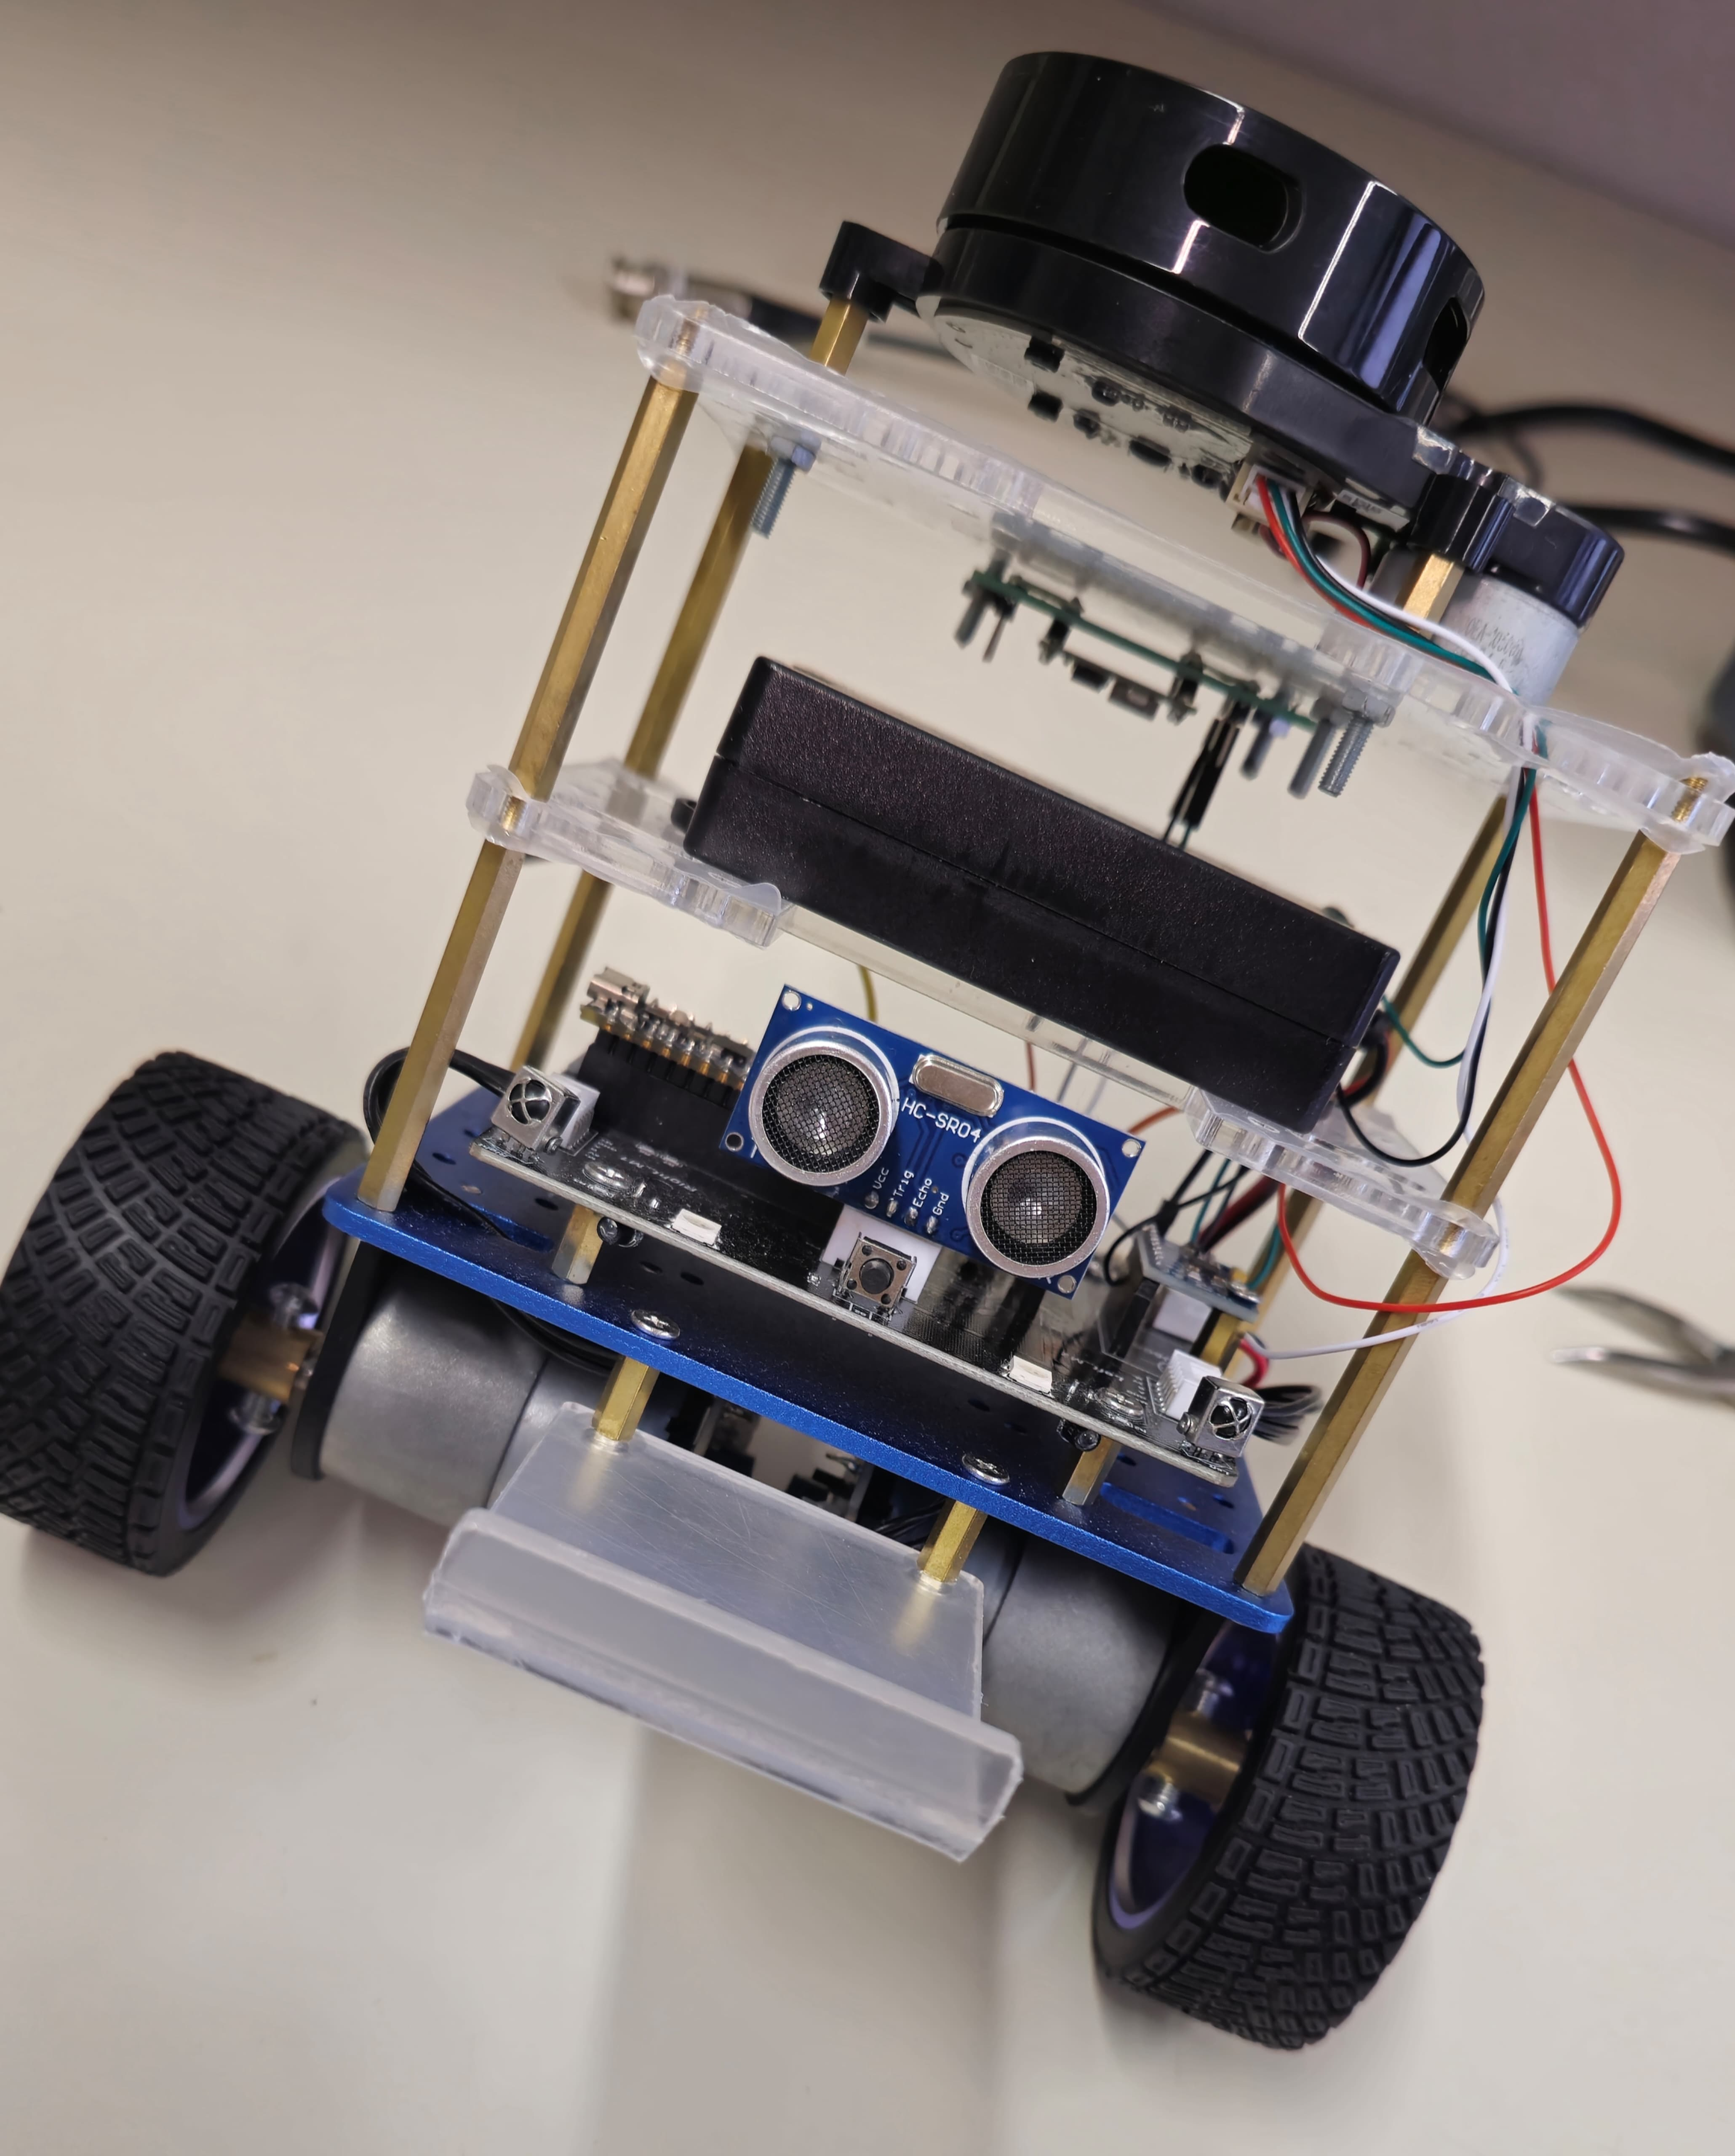
\includegraphics[width=0.8\textwidth]{img/Hardware/guide.jpg}
   \caption{Guide-Roboter}
    \label{fig:guide}
\end{figure}

\subsection{Technische Umsetzung}
\initials{MS}
Damit der Guide die Umgebung erkennen kann, wurde das Fahrgestell des Roboters modifiziert.
%
Die obere Ebene (Akku-Halterung) wurde höher gesetzt, um Platz für den LiDAR-Sensor und seine Halterung zu schaffen.
%
Zusätzlich wurde die Stromversorgung angepasst, indem ein Step-Down-Konverter eingebaut wurde.
%
Dieser liefert die benötigte Spannung für den LiDAR-Sensor.
%
In Abbildung~\ref{fig:guide} ist der verbaute LiDAR-Sensor auf dem Guide-Roboter zu sehen.

\subsection{Einschränkungen}
\initials{MS}
Da der Guide durch den zusätzlichen Sensor schwerer ist, hat er eine etwas kürzere Akkulaufzeit als die anderen Roboter.
%
Außerdem ist der LiDAR-Sensor anfällig für Spiegelungen oder Glasflächen,
weil die Laserstrahlen dort falsch reflektiert werden können.

\section{Tamerlan \& Bambi}
\initials{MS}
\label{subsec:hardware_tamerlan_bambi}

Auch bei Tamerlan und Bambi wurden die originalen Elegoo Tumbller Kits technisch angepasst:
\begin{itemize}
    \item Der Arduino Nano wurde durch ein ESP32-Board im Nano-Format ersetzt.
    \item Das Bluetooth-Modul HC-06 wurde entfernt.
    \item Beide Roboter wurden mit einer ESP32-CAM ausgestattet, um Bilder der Umgebung an den Server senden zu können.
    \item Die Software wurde angepasst, damit sie Daten vom Guide empfangen und darauf reagieren können.
\end{itemize}
In Abbildung~\ref{fig:tamerlan_bambi} sind die beiden Roboter nach dem Umbau zu sehen.
\begin{figure}[H]
    \centering
    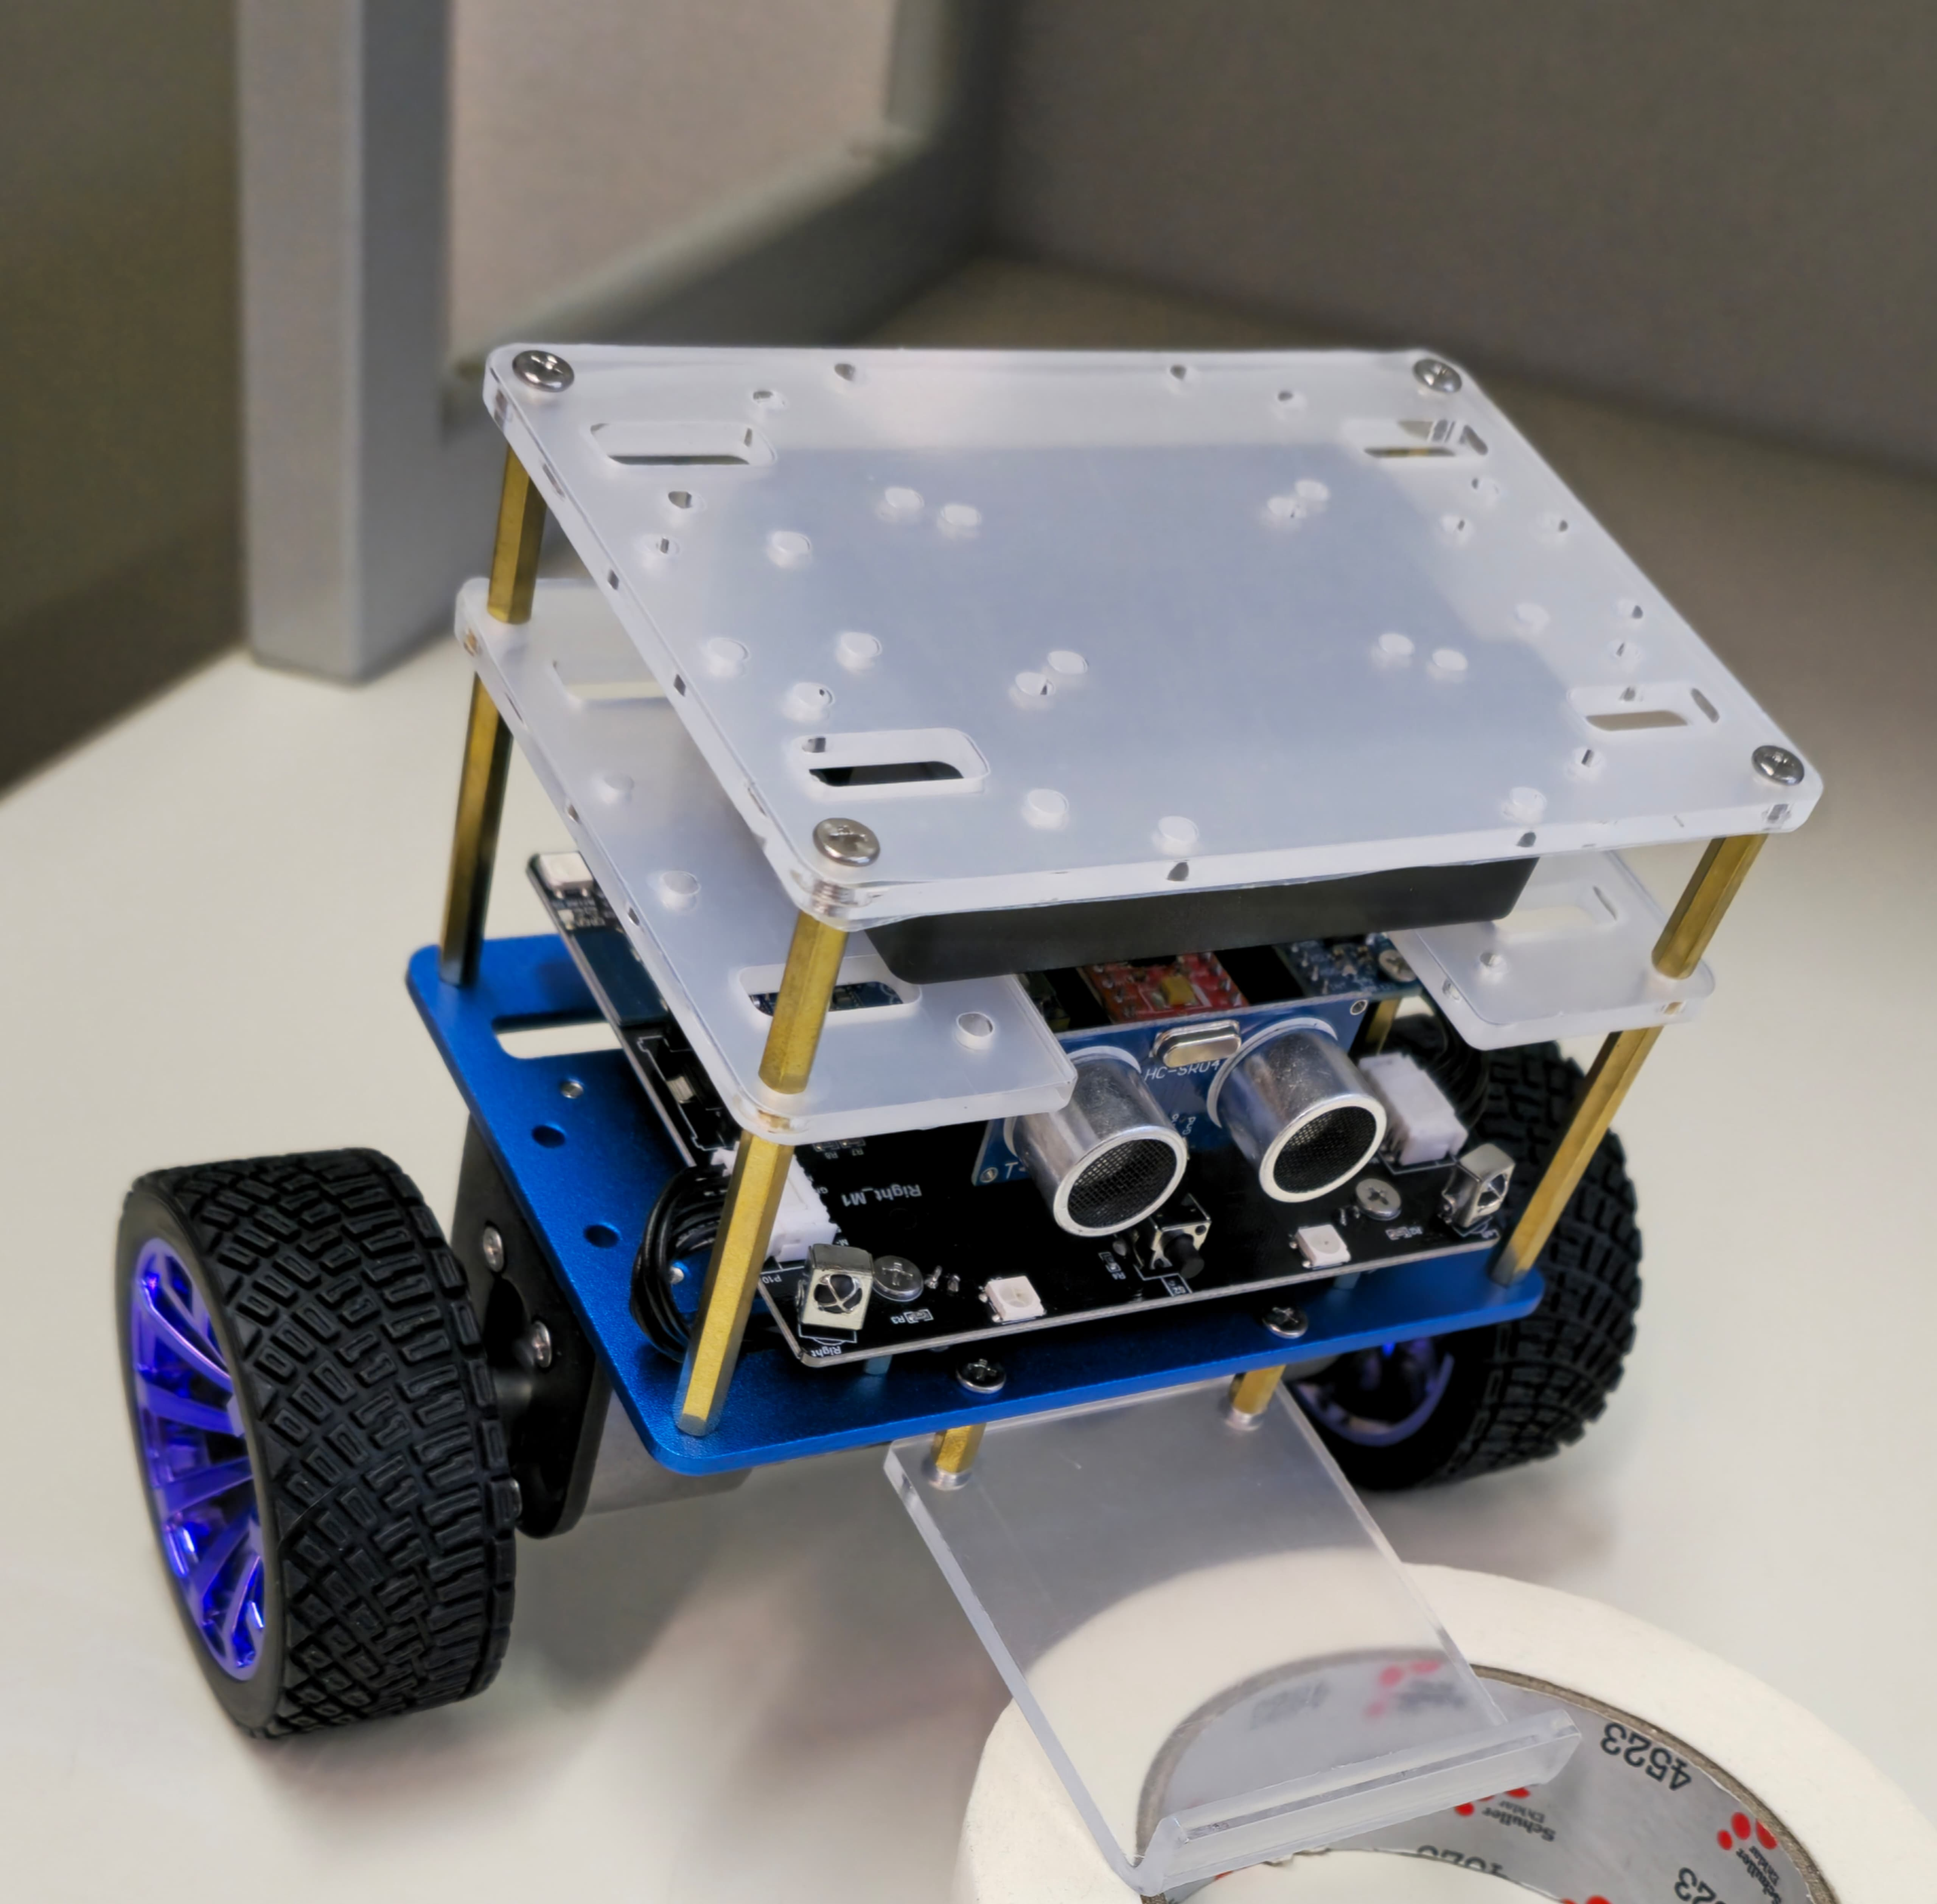
\includegraphics[width=0.7\textwidth]{img/Hardware/tumbler.jpg}
   \caption{Tamerlan und Bambi Roboter}
    \label{fig:tamerlan_bambi}
\end{figure}